\documentclass[conference]{IEEEtran}
\IEEEoverridecommandlockouts
\usepackage{amsmath,
			amssymb,
			amsfonts}
\usepackage{anyfontsize}
\usepackage{mathtools} % ceil, floor
    \DeclarePairedDelimiter\ceil{\lceil}{\rceil}
    \DeclarePairedDelimiter\floor{\lfloor}{\rfloor}
\usepackage{orcidlink}
\usepackage{xfrac} % sfrac


\begin{document}

\title{A Hybrid Technique to Increase Throughput of the Streaming Spectrum Sensor \\
\thanks{This work was supported by the National Aeronautics and Space Administration's (NASA) Space Communications and Navigation Program (SCaN).  This work was performed by NASA Glenn Research Center's (GRC) Cognitive Signal Processing Branch to support NASA's Cognitive Communications Project.}}

\author{\IEEEauthorblockN{Dylan J. Gormley \orcidlink{0000-0002-8140-8248}}
\IEEEauthorblockA{\textit{Cognitive Signal Processing Branch} \\
\textit{NASA Glenn Research Center}\\
Cleveland, OH, USA \\
dylan.j.gormley@nasa.gov}}

% Remember, if you use this you must call \IEEEpubidadjcol in the second column for its text to clear the IEEEpubid mark.
\IEEEpubid{\makebox[\columnwidth]{U.S. government work not protected under U.S. copyright law.}} 

\maketitle

\begin{abstract}
In previous work, there has been significant progress on edge device RF feature detection using a hardware algorithm known as the streaming spectrum sensor (StSS).  Unlike other spectrum sensor implementations, the StSS can function on edge devices due to its low memory requirements.  While the StSS accomplishes its objective of low memory detection, it sacrifices detection throughput.  This work investigates a hybrid technique to balance memory and throughput.
\end{abstract}

\begin{IEEEkeywords}
streaming spectrum sensor, streaming spectral correlation analyzer, RF feature detection, edge computing
\end{IEEEkeywords}

\section{Introduction}
A device that can detect radio frequency (RF) spectrum features, whatever the method, is known as a  spectrum sensor.  The use of this knowledge to improve radio performance is known as cognitive radio (CR).  One common technique of RF feature detection is using what is known as spectral correlation analyzers (SCA).  SCAs estimate a given channel's spectral correlation function (SCF), also called cyclic spectral density (CSD).  Various implementations are available in the literature, such as the SSCA and FAM, each with strengths and weaknesses \cite{gormley-msee21}.

This paper focuses on one implementation method, the streaming spectral correlation analyzer (StSCA).  This method functions on severely resource-constrained platforms, known as edge devices, by estimating the SCF with a focus on memory efficiency.  The results of the StSCA are part of the streaming spectrum sensor (StSS).  The StSS uses peak detection and a threshold on the SCF generated by the StSCA to detect the symbol rate and center frequency offset of active users in a channel.

The original StSCA design is developed in \cite{gormley-msee21}.  The original streaming spectrum sensor design is developed in \cite{gormley-ccaaw21}.  StSS-based applications for CR are discussed in \cite{gormley-ccaaw21} and \cite{dudukovich-rfid22}.  This paper discusses design improvements to the StSS.  It is primarily concerned with adding a preprocessor component to increase throughput at a minimal memory cost.  Also covered in this paper are minor design updates that increase performance, reliability, and resource consumption.  Resource utilization is provided for a sample device.  

\section{Background}
To review \cite{gormley-msee21}, the StSCA output is related to the input by the following equation:
\begin{equation} \label{eq:stsca}
	S_{X}^{v}[k] = \frac{1}{N} \sum_{n=0}^{N-1} {|	X[n]e^{-j2\pi kn}*h[n]|}^{2} e^{-j2\pi vn}.
\end{equation}

Derivation of this equation and a further discussion of its notation can be found in \cite{gormley-msee21}.  The output $S_{X}^{v}[k]$ is the SCF point corresponding to inputs $(X,v,k)$.  The StSS compares the results of the StSCA to the threshold (\ref{eq:cfd}), which results in a list of detected RF features.

\begin{equation}\label{eq:cfd}
  	{|S^{v}_{X}[k]|}^{2}
  	\underset{H_{0}}{\overset{H_{1}}{\gtrless}}
  	\beta \Bigg(\frac{1}{N} \sum_{n=0}^{N-1} {|X[n]|}^{2}\Bigg)^{2}.
\end{equation}

The StSCA was designed to detect symbol rates and center frequency offsets for M- Quadrature Amplitude Modulation (QAM).  Though not tested, it should theoretically work for a wide range of modulations, pulse-shape filters, and line encodings.  Further discussion and definitions can be found at \cite{spooner-SCFs}.

% must be in the second column of the first page, where ever that may be
\IEEEpubidadjcol

\section{Design Overview}

\subsection{New Component:  Symbol Rate Preprocessor (SRP)}
The objective of the original StSCA was to avoid the use of fast Fourier transform (FFT) components in order to save device block random access memory (BRAM).  Thus, the samples are processed in a streaming fashion instead of FFT blocks.  In this update, we add one FFT component as a preprocessor to improve the speed of the StSCA.  Since this is the addition of only one FFT, as opposed to an array of FFTs, such as those used in other SCA implementations, the memory use is still low and suitable for edge devices.  The original StSCA estimates the entire SCF at every symbol rate and center frequency pair.  By adding an SRP, we instead only process symbol rates of interest, and that is, symbol rates that exceed our optimal threshold.

In Fig. \ref{fig:srp_ex} we find that every point of the SCF has been estimated for a given channel.  Realistically, only the symbol rates that exceed the threshold should be passed to the StSCA for processing.  In this example, 11 symbol rates have been calculated, but only two exceed the threshold.  Therefore, only two symbol rates should be further processed using the StSCA.  Assuming no parallelization, the preprocessor increases the system's throughput by a factor of nine.

\begin{figure}[htbp]
\centerline{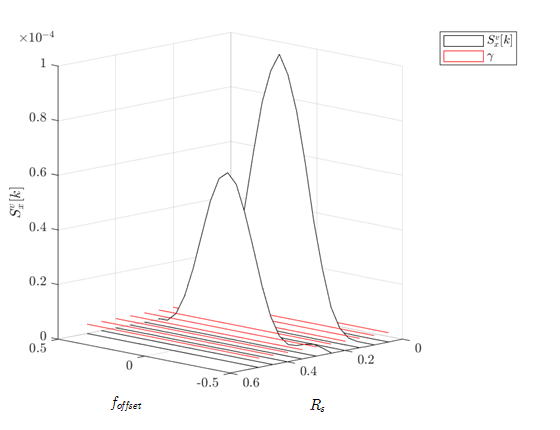
\includegraphics[width=0.5\textwidth]{figs/srp_ex.png}}
\caption{In this example SCF there are two co-channel users.  The first has RF features $(R_{s}=0.1MBd,F_{offset}=-0.2MHz)$.  The second has RF features ${R_{s}=0.25MBd,F_{offset}=0.2MHz}$.}
\label{fig:srp_ex}
\end{figure} 

In Fig. \ref{fig:srp}, we use the new SRP component to calculate the discrete cyclic autocorrelation function (CAF) evaluated at $\tau=0$.  This special case of the CAF simplifies to the form of a DFT, but with a magnitude-squared input and is written as

\begin{equation}\label{eq:caf}
R[v]=R^v_{X}[0]=\frac{1}{N} \sum_{n=0}^{N-1} |X[n]|^{2} e^{-j2 \pi vn}.
\end{equation}

Derivation of this equation can be found in \cite{gormley-msee21}.  Computing the DFT using an FFT algorithm must store $N$ values before producing the result, which consumes large amounts of BRAM.  However, even with this BRAM consumption, a single FFT is much more memory efficient than alternative SCA methods.  A block diagram of the digital design is shown in Fig. \ref{fig:srp}.

\begin{figure}[htbp]
\centerline{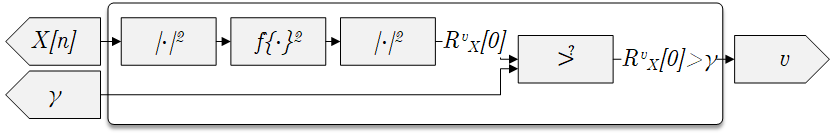
\includegraphics[width=0.5\textwidth]{figs/SRP.png}}
\caption{Unlike the symbol rate estimator from \cite{gormley-msee21}, which processes a single-term DFT instances serially, the SRP processes all terms using a $N$-point FFT.}
\label{fig:srp}
\end{figure}

In the last section of this paper, we will show that even with this new component, BRAM utilization on a CR remains conservative.  

\subsection{Component Update:  Center Frequency Estimator (CFE)}
Fig. \ref{fig:filt_bank} shows the CFE component, which is also the top-level component for the StSCA.   In simulation of the original StSCA, it was found that a static filter of two taps was sufficient to force periodogram convergence and provide accurate detection of the center frequency offsets \cite{gormley-msee21}.  During actual hardware experiments, however, it was found that as a result of noise and quantization error, two taps were not sufficient.  This led to the development of a multiplexer to select between low-pass filter (LPF) banks.  A block design of the LPF bank is shown in Fig. \ref{fig:filt_bank}.

\begin{figure}[htbp]
\centerline{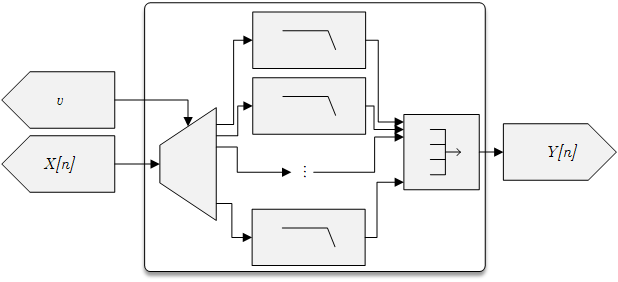
\includegraphics[width=0.5\textwidth]{figs/filt_bank.png}}
\caption{A bank is selected by $v$ and corresponds to an LPF cutoff $v$. Alternatively, using a subset of filter banks instead of a one-to-one match of $v$ to $f_{cutoff}=v$ is a tradeoff between detection accuracy and memory efficiency.}
\label{fig:filt_bank}
\end{figure}

Hardware center frequency offset detection accuracy was dramatically improved using this multiplexer with a small number of taps per LPF.

\subsection{Component Update:  Center Frequency Detector (CFD)}
The CFD component logic has been simplified, but the overall functionality remains the same as the original design developed in \cite{gormley-ccaaw21}.  Previously, the threshold was in this component but has been moved to the StSS component and is utilized in the newly developed SRP.  A block design of the CFD is shown in Fig. \ref{fig:cfd}.

\begin{figure}[htbp]
\centerline{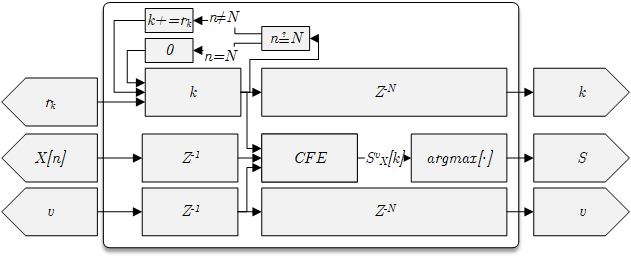
\includegraphics[width=0.5\textwidth]{figs/CFD.png}}
\caption{The CFD generates $k$ using on some step size $r_{s}$, detects the StSCA peak $k$ for some $v$, and to maintain alignments of results.}
\label{fig:cfd}
\end{figure}

\subsection{Component Update:  Symbol Rate Distributor (SRD)}
What was previously called the spectrum sensor component is now called the SRD component.  This component was redesigned from a polling-based distributor in \cite{gormley-ccaaw21} to a one-hot priority encoder-based distributor.  The previous FIFO commutator from \cite{gormley-ccaaw21} was replaced with a one-hot decoder commutator.  Fig. \ref{fig:srd} shows the updated block design.  These updates simplify the logic, increase reliability, and reduce memory consumption.

\begin{figure}[htbp]
\centerline{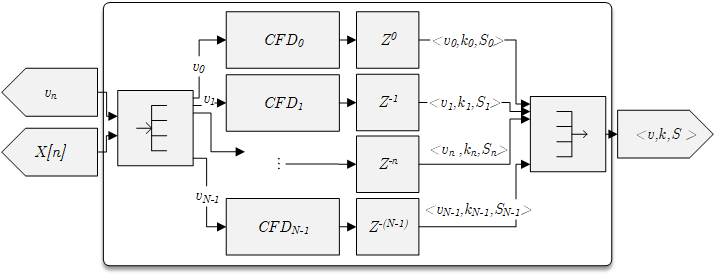
\includegraphics[width=0.5\textwidth]{figs/SRD.png}}
\caption{A symbol rate is fed in from the SRP and passed to a CFD marked \texttt{ready}. If no CFDs are \texttt{ready} at the time of arrival of a new symbol rate, then that $v$ is discarded. CFDs are synchronized to only start at a new when the sample count is $0$. Using this synchronization, each CFD can be delayed equal to its index number, creating output staggering. This allows for commutation of results without needing a buffer or flow control.}
\label{fig:srd}
\end{figure}

\subsection{Component Update:  Streaming Spectrum Sensor}
This component now encompasses the threshold \cite{gormley-ccaaw21}, SRP, SRD, and result FIFOs.  Additionally, this component is tasked with tracking sample and result counts.  The primary function of the streaming spectrum sensor component is still to interact with external components such as the analog to digital converter (ADC) and CPU-based dynamic spectrum manager (DSM).  Fig. \ref{fig:top} shows the redesign of the StSS component.  

\begin{figure}[htbp]
\centerline{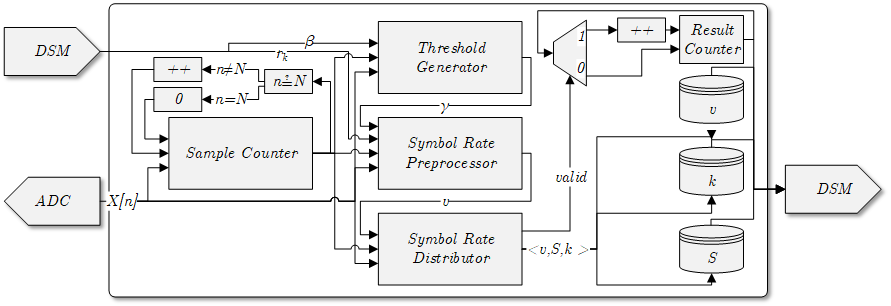
\includegraphics[width=0.5\textwidth]{figs/TOP.png}}
\caption{The DSM sets the probability of false alarm $\beta$, which is used to calculate the threshold. A method to determine the optimal value of $\beta$ is discussed in \cite{gormley-ccaaw21}.}
\label{fig:top}
\end{figure}

Generally, a higher CFD count lessens the need for $\beta$ precision.  The DSM can set the center frequency offset resolution, which is used to iterate through channelizer inputs \cite{gormley-msee21}.  Results are counted and provided to the DSM for CR use, such as those discussed in \cite{dudukovich-rfid22}.

\section{Results}
Results in this section were computed using the Xilinx xc7k7-t, a bit width of $16$, $2^{16}$ samples, and $2$ CFD instances.  Every parallel CFD operation increases \textit{maximum} throughput.  The goal is to select the maximum possible parallel operation size the platform can support while performing its other mission needs, such as baseband processing or interfacing.  For the given parameters, latency is between the start of transmission, and the first result is $34.36s$.  Resource consumption is shown in Tab. \ref{tab:resources}.  As the number of CFDs increases, BRAM consumption grows disproportionately from the other resources.

\begin{table}
\caption{Resource Utilization}
\begin{center}
\begin{tabular}{ |c|c|c|c| }
\hline
Resource  & Used  & Available & Utilization \\
\hline
LUTs      & 22463 & 303600    &  7.40\%     \\ 
Registers & 15426 & 607200    &  2.54\%     \\  
BRAMs     & 186.5 & 1030      & 18.11\%     \\
DSPs      & 284   & 2800      & 10.14\%     \\
\hline
\end{tabular}
\end{center}
\label{tab:resources}
\end{table}

\section{Conclusion}

As discussed in this paper, significant improvements have been made toward a spectrum sensor for edge devices.  There are a few topics that are still open for investigation.  

\begin{itemize}
\item Modeling and simulation suggests that the same threshold should work among various M-QAM parameters but should undergo further experimentation.
\item Replacing the single-term DFT in the StSCA with a Goertzel algorithm may boost performance and reduce resources.
\item The addition of a second threshold based on spectral coherence could further help reduce false alarms.
\item The theoretical bit truncation and rounding values were found to be different from the experimental.
\end{itemize} 

We began this paper with a brief development history of the StSS and its applications for CR.  Following this, we discussed design additions and updates.  In the results section, we found that fabric utilization remains small for nominal parameters, and thus our objective is achieved.

\bibliographystyle{IEEEtran}
\bibliography{IEEEabrv, refs.bib}

\end{document}



